\documentclass{article}
\usepackage[utf8]{inputenc}
\usepackage{tikz,graphicx,hyperref,amsmath,amsfonts,amscd,amssymb,bm,cite,epsfig,epsf}

\title{big data Lecture 2: relational databases}
\author{wbg231 }
\date{January 2023}

\begin{document}

\maketitle

\section{data base management systems}
\begin{itemize}
    
\item DBMS provide
\begin{enumerate}

    \item data integrity and consistency (that is they make sure that data can not be accidentally changed and is correct )
   
    \item concurrent access (that is two people can look at the same file at the same time )
    \item efficient storage and access 
    \item standardized format and methods of administration 
    \item standardized query interface (sql)
\end{enumerate}
\item there are many types of data base management systems (relational, semi-structured, object oriented, object relational etc)
\subsection*{the relational model}
\item data is organized into tables called relations
\item each column represents a set of possible values 
\item a relation over sets $A_1\cdots A_n$ is a subset of there cartesian product
\item the row of a table are known as tuples
\item any columns could take finite or infinite number of values
\item a relation does not need to have all elements of the cartesian product it is just a subset 
\item  relations are the abstract model of the data 
\item tables are explicably constructed relations
\item a view is a relation defined implicitly and constructed dynamically at run time 
\item temporary tables are the output of queries
\item tuples are un ordered 
\item tuples must be UNIQUE
\item there is usually a key for which tuples can not have all of the same  values
\item \textbf{Slido question} if A has 5 elements and B has 3 and $A\cap B = \emptyset$ how many possible relations exist using A 
\item let $R\subset A\times B$  be a relation we know that $|A\times B|=15$ and and R is teh power set of that so $2^{15}$ could also be $(2^{15}+2^{15}-1)$ if we say the order of product matters
\item a relation is defined by a schema 
\item it can be tough to consider all edge cases when making a schema
\item \textbf{slido} what constraints could/should one consider when adding customer name to a field to ensure data integrity
\item this is a really hard question and there is not really a good solution, could hurt difference groups 
\subsection*{relational data base}
\item structured data can be encoded by joining relations on \textcolor{green}{a shared attributes}
\item the collection of schema defines your data model 
\item keys determine the identity of a row 
\item simple keys (one column), compound keys (multiple columns)
\item can also have primary and alternate keys
\subsection*{foreign keys}
\item a key form one relation can be used as a column in another relation called a \textcolor{red}{foreign key}
\item this makes sure that things are consistency between tables
\item this is not automatic and must be ensured in the schema definition 
\subsection*{normalization}
\item \textcolor{red}{a normal database} does not have any redundant information stored.
\item this makes it easy to update data, as you only need to update a record in one place
\item but it can also be tough since it requires a lot joints to get complex queries
\item schema provide a degree of safety and validation 
\section*{sql}
\item sql is the language we use for databases it is \textcolor{red}{declarative} ie we state what we want not how we compute it 
\item that is not the same as C or python which are \textcolor{red}{procedural language} 
\item think of sql as a protocol not a language
\item typically iterate over rows in your host language using select statement 
\item we combine relations by joining data 
\item always run queries with parameters not variables to avoid SQL injection  
\subsection*{types of joints}
\item cross join all combinations of rows (ie the cartesian product)
\item left outer join, right outer join, full  outer join: all rows are retained from one or both relations even if no match is found missing data is stored as null
\item inner join: only matching rows are retained (like an outer join with out nulls)
\item natural join (rows must match on all shared columns this is a a spacial case of inner join)

\subsection*{aggregation}
\item aggregation lets us summarize multiple tables into a single result 
\item these are group by statement ex Select zip, AVG(height) from people group by zip
\item list of aggregation 
\begin{enumerate}
    \item avg, sum min, max
    \item count(distinct X) number of unique values in col x 
    \item count(*) number of rows 
    \item count(x) number of non now rows in col x 
    \item $group_concat(X)$ concatenate string  
\end{enumerate}
\subsection*{ indexing}
\item relational databases store data as a list of tuples but this may not be the best way to store things 
\item if we know how the data will be used we could tell it if the data should be stored in a certain way or what data type to use for storage
\item \textcolor{red}{an index} is a data structure over one or more columns that can accelerate queries
\item an example could be if you know you are going to be grouping by col value, in a lot of searches then indexing by that col value could be faster than just running without the index
\item there are some drawbacks of indexing though 
\begin{enumerate}
    \item they take time and space to construct 
    \item updated becomes slower since you also need to update the index 
    \item there is no guarantee they will actually speed things up
\end{enumerate}
\item when is it good to index
\begin{enumerate}
    \item when data is read more often than written 
    \item when queries are predictable 
    \item when queries rely on a small number of columns
    \item indexes can be added or deleted as needed 
\end{enumerate}
\section*{integrity }
\item file systems can not preform actions simultaneously which can make them have inconsistent results
\item file systems can not handle concurrent file updates, ie two people could be reading or writing to one file at the same time which can lead to bad results 
\item WE more or less want our DBMS to be ACID compliant 
\subsection*{ACID}
\item Atomicity ie operations are all or nothing (there are no partial updates operations are bundled in transactions (ie groups of updates)) 
\item consistency updates must move from one valid state to another 
\item isolation concurrent operations do not depend on order of execution 
\item durability compiler transactions are permanent once a transaction is completed push it to disk 
\subsection*{Atomicity in practice}
\item basically have a try except statement that if a transaction is successful we commit it, otherwise we roll back (so if something fails we just go back to a valid state )
\subsection*{transaction example}
\item 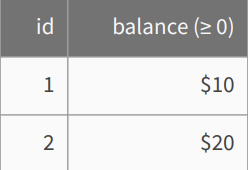
\includegraphics[width=10cm]{/Users/hochwagenlab/Desktop/buz/school/big-data-spring-2023/review/week_2/lecture/images/l2_1.png}
\item imagine we have the above table 
\item we can not transfer 20 from account 1 to account 2, since that would make account 1 negative 
\subsection*{consistency}
\item consistency is maintained by a schema in practice (schemas specificity values for there columns)
\subsection*{isolation in practice}
\item usually achieved by lacking the database during modification
\item this is really important for distributed systems 
\item \textcolor{purple}{git } is ACID compliant
\item \subsection*{slido question} what if we want to add a new edge and node to a graph that must always be connected which acid property would most easily fix this? Atomicity
\end{itemize}
\end{document}
